\chapter{Theory}\label{chapter:theory}

This chapter explains the theoretical concepts needed to understand the \textit{natural language processing} (\textit{NLP}) system described in the next chapter. This chapter is broken down into two parts. The first part explains some common terms used in NLP and the second part of the chapter explains \textit{support vector machines} (\textit{SVM}).

\section{Natural Language Processing (NLP)}

Natural Language Processing (NLP) is an area of research and application that explores how computers can be used to understand and manipulate natural language text or speech to do useful things \cite{chowdhury2003natural}. The foundations of NLP lie in a myriad of disciplines, viz. computer and information sciences, formal language theory, linguistics, artificial intelligence, psycho-linguistics, etc.

\subsection{NLP Basics}\label{sec:NLPPipeline}

NLP systems work on a chunk of text as input. However, plain text data is unstructured data and all NLP systems preprocess the data in order to convert it into a structured representation. There are two types of tasks in NLP, viz. syntactic tasks and semantic tasks \cite{nlpcourse}. All NLP systems work on many of these tasks in order to achieve a certain objective.

Syntax relates to the proper ordering of the words and its effect on the meaning, while semantics deals with the literal meaning of the words, phrases and sentences \cite{wiki:sentSeg}. This section presents an overview of syntactic tasks. Most of the NLP systems use syntactic tasks for preprocessing the data.

\subsubsection{Sentence Segmentation}

\textit{Sentence segmentation} is the process of dividing a chunk of text into component sentences \cite{wiki:sentSeg}. In English and some other languages, \emph{segmenting} after a fullstop ('.') is a reasonable approximation. However, the problem is not so trivial due to the use of abbreviations such as "Mr.", due to decimal numbers such as "3.1416", etc. For example, in the sentence \textit{"Mr. Smith went to the shops in Jones Street."}, the sentence actually ends after the word \textit{"Street"} and not after the abbreviation \textit{"Mr."}. In other languages, like Chinese, the task is more complex since they do not have a proper punctuation character that can be used for approximating sentence boundaries.

\subsubsection{Word Segmentation}

\textit{Word segmentation} is the process of dividing text into constituent words \cite{wiki:sentSeg}. Usually, white spaces can be used to parse the text into words in English. Although white spaces are a good approximation, sometimes they are not present. For example, the word \textit{couldn't} consists of two words \textit{could} and \textit{not}, which cannot be split using a white space. In some other languages like Chinese, words are not separated by spaces

\subsubsection{Tokenization}

\textit{Tokens} are the smallest processing unit in NLP systems. In most cases, a token is the equivalent of a word. In other cases, for instance, the word \textit{couldn't} could be \emph{tokenized} into multiple tokens, such as: \textit{couldn}, \textit{'}, and \textit{t}. In other NLP systems, a token can also be a sentence or a paragraph. Therefore, the tokenization algorithm depends on the NLP task to solve.

\subsubsection{Stemming and Lemmatization}

\textit{Stemming} and \textit{lemmatization} are the processes used to reduce a word to its \textit{base} form. Such reductions are useful for NLP systems. However, there is a difference between \textit{stemming} and \textit{lemmatization}. \textit{Stemming} refers to the crude heuristic process of chopping off the ends of the words in hope of finding the base word \cite{stemminglemmatization}. This works most of the time. For example, the stem of words \textit{running} and \textit{runs} is \textit{run}. \textit{Lemmatization} usually extracts the base word properly with the use of a vocabulary and morphological analysis of the words \cite{stemminglemmatization}.  This requires knowledge of the specific treated language. For example, the base of \textit{is}, \textit{am} and \textit{are} is \textit{be} which can only be extracted by lemmatization and not by stemming.

\subsubsection{Part-Of-The-Speech (POS) Tagging}

\textit{Part-of-the-speech (POS) tagging} is the process of annotating each word in the sentence with a \textit{part-of-the-speech tag}. The common examples of POS tags are \textit{noun} and \textit{verb}. This is an important step and is useful for subsequent syntactic parsing and word sense disambiguation \cite{nlpcourse}. 

\subsubsection{Parsing}

There are two views of linguistic structure in NLP, viz., \textit{constituency} (phrase structure) and \textit{dependency structure} \cite{parsing}. Both structures are represented as trees. The process of producing these structures correctly is called \textit{parsing}. There are two types of parsing:

\begin{figure}
\centering
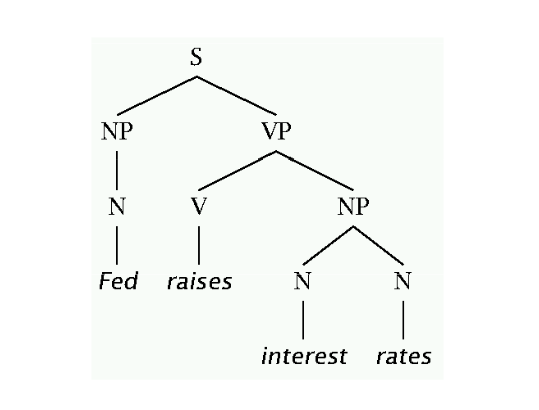
\includegraphics[scale=0.5]{figures/SyntacticParse.png}
\caption{An example of constituency parsing.}\label{fig:SynParse}
\end{figure}

\begin{figure}
\centering
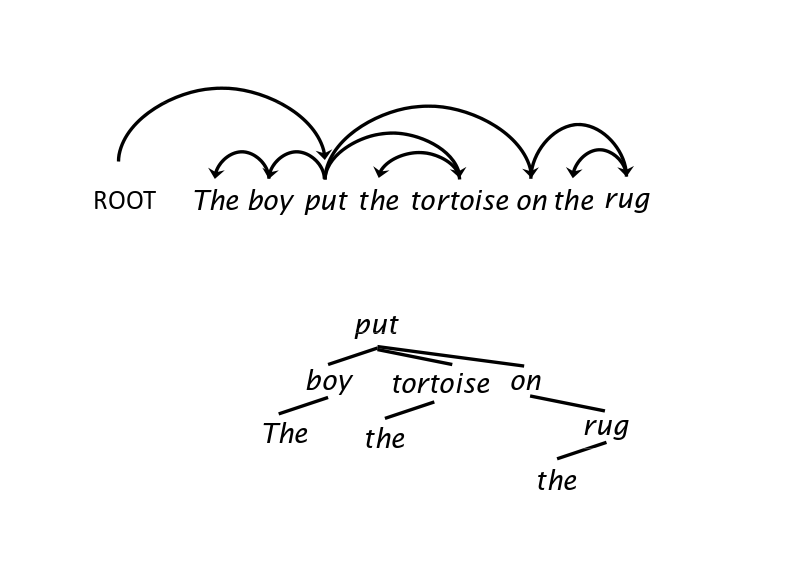
\includegraphics[scale=0.4]{figures/DependencyParse.png}
\caption{An example of dependency parsing.}\label{fig:DepParse}
\end{figure}


\begin{itemize}

\item \textit{Constituency parsing:} is the process of producing a constituency structure from a sentence. Following the rules of phrase structure grammar \cite{wiki:phrasegrammar}, the words in the sentences are grouped into components called constituents. These constituents are then nested to form a constituency structure. Fig. \ref{fig:SynParse} shows the constituency structure of the sentence \textit{"Fed raises interest rates."}.

\item \textit{Dependency parsing:} is the process of producing a dependency parse/structure from a sentence. In dependency parsing, the binary relations among the words are used to create a dependency parse tree. In a dependency tree, the words in the sentence act as nodes and the dependency relations between them act as edges. Fig. \ref{fig:DepParse} shows the dependency parse of sentence \textit{"The boy put the tortoise on the rug."}.

\end{itemize}

\subsection{NLP Pipeline}

Most NLP systems are a complex pipeline of NLP sub-tasks. For any processing to be done, it is necessary to break down the unstructured text input into structured units. Most of the syntactic tasks mentioned in the previous section are used for preprocessing the text. The usual pipeline for an NLP system looks like as shown in the Fig. \ref{fig:NLPPipe}.

\begin{figure}
\centering
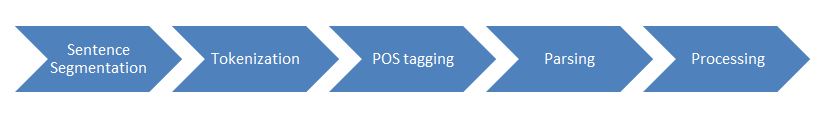
\includegraphics[scale=0.4]{figures/NLPPipeline.png}
\caption{Usual NLP pipeline.}\label{fig:NLPPipe}
\end{figure}

\subsection{NLP Semantic Tasks}

Semantic tasks in NLP deal with extracting meaningful information from the text. Following are different types of semantic tasks:

\subsubsection{Named Entity Recognition (NER)}

Named entities are atomic elements in the text belonging to predefined categories \cite{ner1}, such as the names of persons, organizations, locations, etc. In simple words, \textit{named entity recognition (NER)} is the task of taking an unannotated block of text such as \textit{"Jim bought 300 shares of Acme Corp. in 2006."} and converting it into an annotated block like \textit{"$[Jim]_{Person}$ bought 300 shares of $[Acme Corp.]_{Organization}$ in $[2006]_{Time}$."} \cite{wiki:ner}.

\subsubsection{Machine Translation}
% Search Engines
% Helping the human translators

\textit{Machine translation} is the process of translating text or speech from one language to another automatically without human intervention.

\subsubsection{Relationship Extraction}\label{sec:RE}
% task of extracting information from emails

\textit{Relationship extraction} is the process of identifying relationships between different named entities present in the sentence. For example, in the sentence \textit{"$TUM_{university}$ is located in $Munich_{location}$"}, \textit{TUM} and \textit{Munich} are connected by the relation \textit{located-in(TUM,Munich)}.

\subsubsection{Coreference Resolution}

\textit{Coreference resolution} is the task of finding all expressions that refer to the same entity in the text. For example, in the sentence \textit{"Sally arrived, but nobody saw her."}, both \textit{her} and \textit{Sally} refer to the same entity.

\subsubsection{Other Semantic Tasks}
% Other tasks: 
% 2. word sense disambiguation 
%4. Question Answering 
%5. Document summarization 
%- summary of an article
%6. Dialog
%- Human machine communication

There are a plethora of other semantic tasks in NLP such as sentiment analysis, spam detection, information extraction, question answering, word sense disambiguation, document summarization, etc.

\section{Support Vector Machines}\label{sec:SVM}
% Write about some of the theory behind SVM

Machine Learning algorithms are algorithms that can learn patterns from data. Machine learning tasks can be broadly classified into \textit{supervised learning} and \textit{unsupervised learning}. In supervised learning, the algorithms are given a set of data along with their labels and the goal for algorithms is to learn a function that maps the input data to their correct \textit{given} labels. In unsupervised learning, the goal is the same, however, the training data is given without assigned labels and so the algorithms must assign the correct \emph{implicit} labels.

Support vector machines (SVM) are supervised learning models that can be used for the task of classification and regression. SVMs are widely used for the task of classification, i.e., classifying the data into predefined classes/labels.

\subsection{Mathematical Formulation}
\begin{figure}
\centering
\begin{minipage}{.5\textwidth}
  \centering
  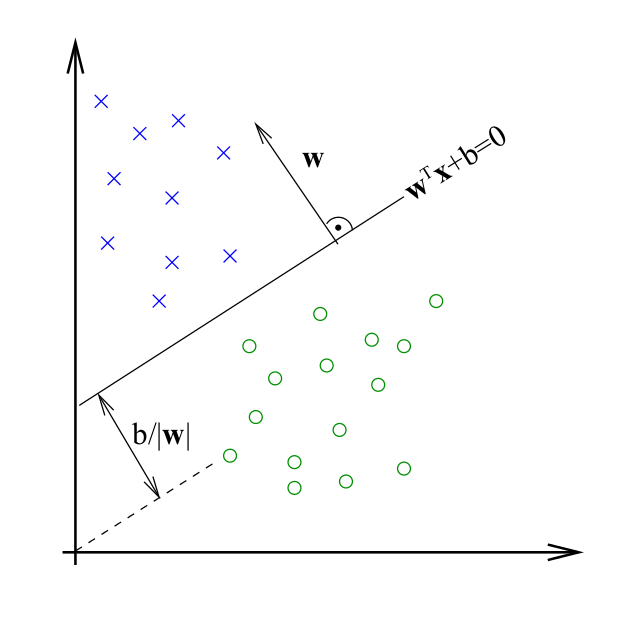
\includegraphics[width=.95\textwidth]{figures/SVMFigure1.png}
  \caption{Data separating hyperplane.}
  \label{fig:SVM1}
\end{minipage}%
\begin{minipage}{.5\textwidth}
  \centering
  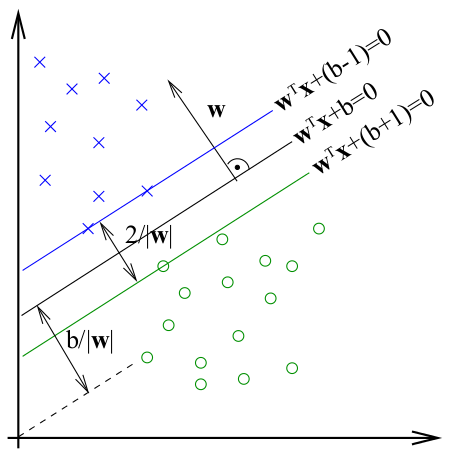
\includegraphics[width=.95\textwidth]{figures/SVMFigure2.png}
  \caption{Maximum margin classifier.}
  \label{fig:SVM2}
\end{minipage}
\end{figure}

%\begin{figure}
%\centering
%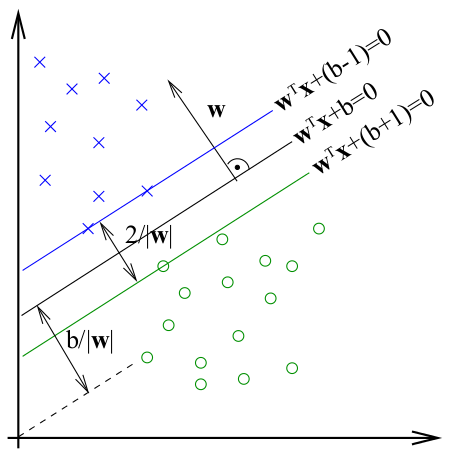
\includegraphics[scale=0.4]{figures/SVMFigure2.png}
%\caption{Maximum margin classifier}\label{fig:SVM2}
%\end{figure}
%
%\begin{figure}
%\centering
%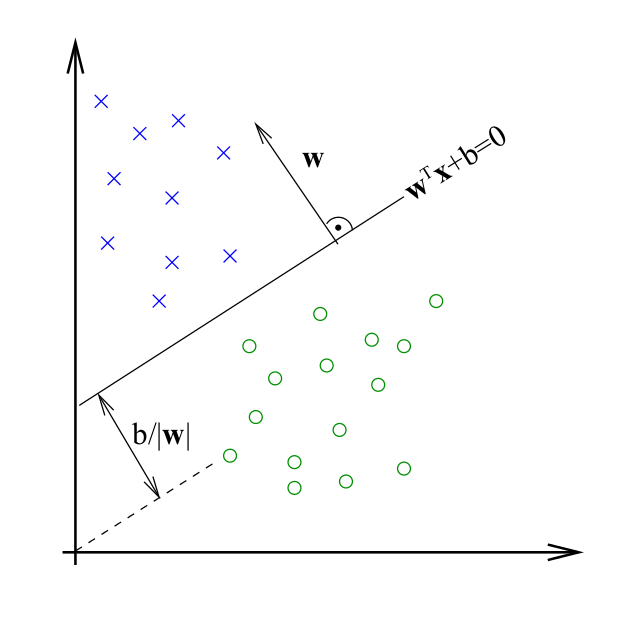
\includegraphics[scale=0.4]{figures/SVMFigure1.png}
%\caption{Hyperplane separating data points}\label{fig:SVM1}
%\end{figure}


SVMs try to build a hyperplane that best separates the data points belonging to two different categories. For example, as shown in Fig. \ref{fig:SVM1}, the hyperplane separating the blue points and green points is given by:

$$
\mathbf{w}^{T}\mathbf{x} + b = 0
$$

where $\mathbf{w}$ is a vector normal to the hyperplane, $b$ is a constant and  $\mathbf{x}$ is the set of all points, that satisfy above equation and are located on the hyperplane. The vector $\mathbf{w}$ is also called a weight vector. The projection length from the origin is denoted by $\frac{b}{|\mathbf{w}|}$. 

For a point $\mathbf{x}_1$ having projection length greater than $\frac{b}{|\mathbf{w}|}$, $\mathbf{w}^{T}\mathbf{x}_1 + b > 0$ and the point is classified as a blue point. Similarly, for a point $\mathbf{x}_2$ having projection length less than $\frac{b}{|\mathbf{w}|}$, $\mathbf{w}^{T}\mathbf{x}_2 + b < 0$ and the point is classified as a green point. Therefore, the class of a new point $\mathbf{x}$ is given by:

\begin{align}
\begin{aligned}
%$$
h(\mathbf{x}) = sgn(\mathbf{w}^{T}\mathbf{x} + b) \label{eq:sgn}
%$$
\end{aligned}
\end{align}

Intuitively, the greater the distance of the points on each side of the hyperplane, the better the classification. Therefore, efforts are made to construct a maximum margin classifier.  Such a classifier will make it more likely to classify a new point on the right side of the dividing hyperplane. Hence, the problem of constructing a hyperplane is refined to constructing a hyperplane that separates both classes and has maximum margin.

Figure \ref{fig:SVM2} shows an maximum margin classifier such that the size of the margin is given by:

$$
m=\frac{2}{|\mathbf{w}|}
$$

For such a classifier, if the target classes for data point $\mathbf{x}_i$ are given by $\mathbf{y}_i \in \left\lbrace -1, +1 \right\rbrace$, then the constraints

\begin{align}
\begin{aligned}
\mathbf{w}^{T}\mathbf{x}_i + b \geq +1 \quad \text{for} \quad y_i = +1 \\
\mathbf{w}^{T}\mathbf{x}_i + b \leq -1 \quad \text{for} \quad y_i = -1
\end{aligned}
\end{align}

can be condensed into 

$$
y_i (\mathbf{w}^{T}\mathbf{x}_i + b) \geq 1 \quad \text{for all} \quad i
$$

Therefore, the problem of finding a maximum margin classifier can be formulated as a constrained convex optimization problem as follows:

\begin{align}
\begin{aligned}
\text{minimize} \quad f_0(\mathbf{w},b) &= \frac{1}{2} \mathbf{w}^{T} \mathbf{w} \\
\text{subject to} \quad f_i(\mathbf{w},b) &= y_i (\mathbf{w}^{T}\mathbf{x}_i + b) -1 \geq 0 \quad \text{for} \quad i = 1,...,m
\end{aligned}
\end{align}

Upon solving the optimization problem, the weights are found to be linear combination of training samples:

$$
\mathbf{w} = \sum^{m}_{i=1} \alpha_i y_i x_i
$$

Substituting the weight vector into equation \ref{eq:sgn}, the class of a new point $\mathbf{x}$ is given by:

$$
h(\mathbf{x}) = sgn(\sum^{m}_{i=1} \alpha_i y_i x_i^{T} x_i + b)
$$

\begin{figure}
\centering
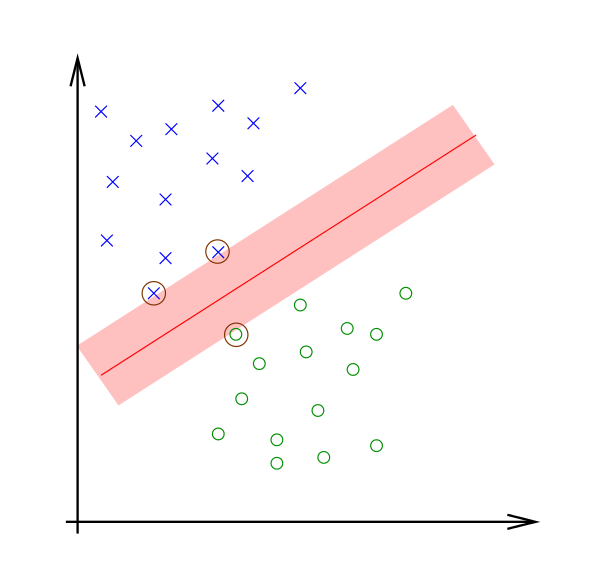
\includegraphics[scale=0.4]{figures/SVMFigure3.png}
\caption{Maximum margin hyperplane along with support vectors (encircled points).}\label{fig:SVM3}
\end{figure}

Actually, only the data points lying on the margin contribute to the weight vector and are therefore called \textit{support vectors}. The support vector points are encircled in the figure \ref{fig:SVM3}. 

\subsection{Training, Testing and Overfitting}

The process of building a maximum margin classifier using training samples is known as \textit{Training}. Once the classifier is built, the process of using this classifier for classification of unseen test samples is called \textit{Testing}. 

\textit{Training error} and \textit{Test error} are the metrics used for calculating the performance of classification on training samples and test samples, respectively. In case of low training error, it may happen that the hyperplane classifies all the training samples with very high accuracy but fails to classify testing samples correctly. In other words, the support vector machine model fits perfectly for training samples but does not generalize. This phenomenon of fitting only to the training samples is called \textit{Overfitting}.

\subsection{Regularization Parameter} \label{subsec:RegPar}

One of the hyperparameters used in support vector machines is known as regularization parameter and denoted by $\mathbf{C}$. Regularization parameter controls the trade off between achieving a low \textit{training error} and achieving a low \textit{testing error}. It tells the SVM optimization how much it should avoid misclassifying each training example. In other words, using large values of $\mathbf{C}$ may fit the training data very well and can result in overfitting. On the other hand, small values of $\mathbf{C}$ may lead to lower performance on training set but better generalization.
